% Rapport sur l'environnement de développement avec Vagrant
\documentclass[12pt,a4paper]{article}

\usepackage[francais]{babel}
\usepackage[utf8]{inputenc}
\usepackage[T1]{fontenc}
\usepackage{graphicx} % Pour intégrer des images
\usepackage{hyperref} % Liens externes
\usepackage{listings} % Code source
\usepackage{hyperref} % Lien hypertexte

\usepackage{vmargin} % Pour formater la taille des marges du doc
\setpapersize{A4}
\setmargins{20mm}{15mm}{170mm}{250mm}{10mm}{0mm}{0pt}{1.2cm}

\title{Les environnements de développement avec Vagrant et Docker}
\author{Maxence Bothorel, Thibaut Crouvezier}
\date{22/01/2015}

\begin{document}

\maketitle{}

\begin{center}
  
\includegraphics[width=10cm]{images_rapport/univ_logo.jpg}
\end{center}

\newpage{}

\tableofcontents{}

\newpage{}

\section{Introduction}
Un environnement de développement est un ensemble d'outils et de logiciels afin d'augmenter la productivité d'un développeur. Cela peut être un éditeur de texte, avec un débogeur et un compilateur. Dans notre cas, l'environnement de développement est une plateforme qui sert au développeur à essayer ses logiciels, dans un environnement cloturé afin de ne pas porter atteinte à son système en cas d'erreurs. L'environnement est de préférence portable, afin que plusieurs développeurs puissent travailler avec la même base. Nous verrons deux pionniers dans le domaine : Vagrant et Docker. Nous étudierons leurs utilisations et leurs configurations  après avoir rappelé leurs concepts, la virtualisation et les conteneurs. 

\section{Rappels}

\subsection{Qu'est-ce que la virtualisation ?}

La virtualisation est le fait de créer une "machine virtuelle", un nouveau système d'exploitation qui s'exécutera au dessus du système principal. On dit que la machine hôte est celle ou la machine invitée est virtualisée. Cette machine virtuelle est indépendante du matérielle.

Le système invité est entièrement indépendant de l'hôte, ce qui permet de virtualiser un Microsoft Windows 7 sur Debian 8, ou l'inverse. Ce système a ses limites. En effet, il est gourmand en ressources (processeur, RAM) puisqu'il faut disposer d'assez de puissance pour faire fonctionner plusieurs systèmes d'exploitations.

\begin{center}
  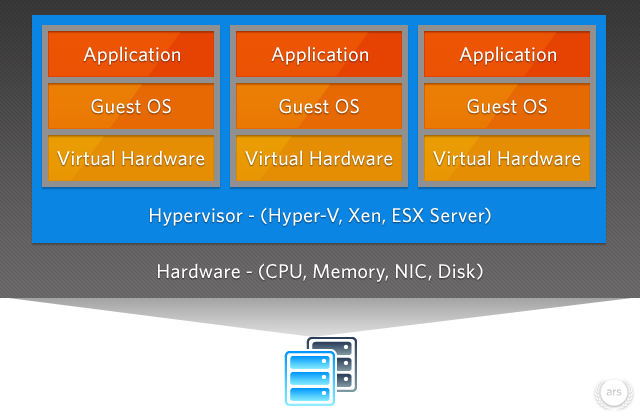
\includegraphics[width=15cm]{images_rapport/virtualisation.jpg}
\end{center}

Sur l'image ci-dessus, On peut voir le matériel en gris, puis l'hyperviseur en bleu, c'est à dire le système hôte. On voit également qu'il y a trois systèmes invités, avec leurs applications. On voit clairement que les systèmes invités sont indépendants du matériel de la machine, puisqu'il est également virtualisé. On peut décider de créer un ensemble de matériel virtuel, comprenant un disque dur virtuel de 20Go, un processeur avec 2 cores et 4Go de RAM afin qu'une machine puisse fonctionneer

\subsection{Qu'est-ce que la virtualisation par conteneurs ?}

La virtualisation par conteneurs ne nécessite pas de virtualiser un système d'exploitation complet, il se charge juste d'empaqueter un environnement de développement léger pour le déploiement d'applications. Ce système de virtualisation est dépendant du système hôte et des conteneurs entre eux. 

\begin{center}
  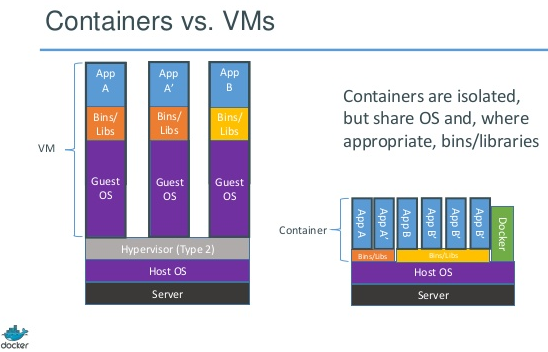
\includegraphics[width=15cm]{images_rapport/vm_container.jpg}
\end{center}

La désavantage de cette virtualisation est qu'elle se base sur le noyau du système hôte, ce qui restreint son déploiement. Il faut donc un conteneur Linux pour un noyau Linux. 

De l'autre coté, cette dépendance au noyau, permet une meilleure gestion des ressources. En effet, la virtualisation par conteneurs permet de pouvoir exploiter toute la quantité de RAM de l'hôte, ainsi que tous ces processeurs.

\section{Vagrant}

\subsection{Introduction}
\begin{center}
  
\includegraphics[width=12cm]{images_rapport/vagrant_logo.jpg}
\end{center}

\textbf{Vagrant} est un outil développé en Ruby, sous licence MIT pour créer des environnements de développements. Il se veut simple d'utilisation afin d'augmenter la productivité de l'utilisateur. Le développement de Vagrant à commencer en Janvier 2010 par Mitchell Hashimoto. Celui ci a travaillé sur Vagrant pendant 3 ans sur son temps libre, avant de créer l'entreprise \textbf{Hashicorp}, afin de continuer le projet à plein temps.

Vagrant créé et gère des machines virtuelles à destinations des développeurs. Ces machines permettent à l'utilisateur d'effectuer des tests dans un environnement fermé, afin de ne pas casser son système d'exploitation. 

Vagrant met en place des machines virtuelles sur VirtualBox, VMWare (Fusion et Workstation), dans le cloud grâce à AWS d'Amazon et Openstack, et également dans des conteneurs Docker et LXC. Il est disponnible sur Windows, OS X et Linux. De plus, Red Hat a créé un plugin permettant à Vagrant de fonctionner avec KVM.

Vagrant permet donc de travailler de façon sécurisée, à seul ou à plusieurs afin d'essayer des logiciels, des scripts ou autre...

\subsection{Installation}
Vagrant est dans les dépôts de Debian unstable en version 1.6.5, et est disponnible en version 1.7.2 sur le site officiel. Le projet Fedora ne supporte pas encore Vagrant. Malgré cela, les développeurs souhaitent le proposer pour la version 22 avec le logiciel libvirt comme hyperviseur par défaut, au lieu de VirtualBox.

On peut donc télécharger le tarball sur GitHub, le récupérer grâce aux dépôts sur Debian et ses dérivés. On peut également télécharger les paquêts Deb, RPM, les executables .msi et .dmg pour Windows et OS X sur le site officiel du projet.

Nous avons utilisé les versions disponnible sur Debian unstable et la dernière, disponnible sur le site officiel.

\subsection{Utilisation basique}

Pour créer une nouvelle machine virtuelle, il suffit d'utiliser les commandes :
\begin{lstlisting}
vagrant init ubuntu/trusty64
vagrant up
vagrant ssh
\end{lstlisting}

La première commande sert à créer un Vangrantfile, un fichier de configuration de la machine. La deuxième commande télécharge le disque virtuel hébergé par Hashicorp\footnote{Hashicorp a créé un \href{https://atlas.hashicorp.com/boxes/search}{annuaire de machines}, afin d'en faciliter le téléchargement}, la société derrière Vagrant.
Au bout de quelques minutes, la machine est téléchargée et prête à être utilisée. Un shell est lancé grâce à la dernière commande. 

Lorsqu'une commande de Vagrant est utilisée, celui-ci remonte l'arborescence afin de trouver le Vagrantfile. On peut changer le répertoire à partir duquel Vagrant lance la recherche grâce à la variable d'environnement VAGRANT\_CWD. 

\subsection{Fichiers de configuration}
Les fichiers de configuration de Vagrant sont des Vagrantfiles. Il en existe plusieurs, et sont tous lus dans un certain ordre lors du démarrage d'une machine :
\begin{enumerate}
	\item{Le Vagrantfile téléchargé avec la machine.}
	\item{Un Vagrantfile dans le dossier /home/user/.vagrant.d, qui est appliqué sur toutes les machines.}
	\item{Le Vagrantfile créé lors de la commande d'initialisation de la machine.}
	\item{Si le dernier n'existe pas, un Vagrantfile concernant plusieurs machines.}
	\item{Si le dernier n'existe pas non plus, un Vagrantfile qui concerne l'hyperviseur.}
\end{enumerate}

Les fichiers sont donc lus un par un et les configurations fusionnées ou remplacées. C'est du Ruby (ce qui permet d'en faire des scripts aisément) :
\begin{lstlisting}
Vagrant.configure(2) do |config|
  ...
end
\end{lstlisting}
Le chiffre 2 signifie que la version de configuration est pour Vagrant version 1.1 ou plus, alors que les configurations pour les versions 1.0.x sont mentionnées par un 1.

On peut également obligé l'utilisateur à avoir une certaine version de Vagrant (dans ce cas, une version entre la 1.3.5 et la 1.4.0) :
\begin{lstlisting}
Vagrant.require_version ">= 1.3.5", "< 1.4.0"
\end{lstlisting}

Il existe beaucoup de paramètres de configurations et sont classés comme ceci : 
\begin{itemize}
	\item{Les configurations comprenant config.vm, qui concernent la machine et son disque virtuel (mise à jour, checksum, réseau, hostname...).}
	\item{Les configurations comprenant config.ssh, qui permet à Vagrant de savoir comment utiliser SSH avec la machine (port, clé SSH, utilisation de X11...).} 
	\item{Les configurations comprenant config.winrm, qui permettent à Vagrant de savoir comment accéder à une machine Windows (nom d'utilisateur, mot de passe, port...).}
	\item{Les configurations comprenant config.vagrant, qui concernent le système hôte. Par défaut en détection automatique.}
\end{itemize}

\subsection{Partages}

\subsubsection{Le partage de dossier}
Vagrant permet de partager des dossiers entre l'hôte et l'invité. De base, le dossier partagé est celui où est le \textit{Vagrantfile} sur l'hôte, et \textit{/vagrant} sur l'invité. Le type de partage par défaut est celui de VirtualBox si l'on utilise ce logiciel, mais d'autres existent.

La commande pour la synchronisation des dossiers dans le \textit{Vagrantfile} est\footnote{Le paramètre a été mis sur deux lignes pour éviter qu'il déborde de la page} :
\begin{lstlisting}
 config.vm.synced_folder "src/", "/srv/website", 
 create: true, disabled: false, type: nfs
\end{lstlisting}
On peut voir ci-dessus que lors du prochain redémarrage de la machine :
\begin{itemize}
	\item{Le dossier src/ de l'hôte sera synchronisé avec le dossier /src/website de l'invité.}
	\item{Le dossier de la machine hôte sera créé s'il n'existe pas.}
	\item{Le partage sera activé.}
	\item{Le type de partage sera NFS.}
\end{itemize}
Il existe également les paramètres pour définir le propriétaire du partage, le groupe du partage (tout deux SSH par défaut), et les options de montages.

De plus, d'autres paramètres existent pour le partage NFS : 
\begin{itemize}
	\item{nfs\_export (booléen) : S'il est a false, vagrant ne modifiera pas le fichier /etc/exports utilisé par NFS.}
	\item{nfs\_udp (booléen) : Ce paramètre sert à savoir quel protocole de transport utilisé.}
	\item{nfs\_version (nombre) : Ce paramètre sert à déterminer la version de NFS utilisé.}
\end{itemize}
Pour que Vagrant modifie le fichier /etc/exports, il lui faut des droits root. Il est donc possible de renseigner le mot de passe à chaque démarrage de machine, de mettre vagrant dans le groupe sudoers ou de modifier soi-même le fichier.

Il est également possible de synchroniser les dossiers avec rsync. Dans ce cas, il sera nécessaire d'utiliser rsync-auto afin de synchroniser les dossiers à chaque changements. Le partage via SMB est quant à lui disponnible que pour les hôtes Windows. 

En résumé : le partage via NFS est à privilégier car il est plus performant et a moins d'inconvéniants (un bug de VirtualBox peut entraîner des fichiers corrompus, la synchronisation automatique avec rsync est plus fastidieuse a mettre en place et SMB est disponnible que pour les hôtes Windows).

\subsubsection{Le partage des machines}
Vagrant est un logiciel collaboratif : il est possible de partager ses machines avec n'importe qui. Pour ce faire, vagrant dispose de commandes :
\begin{lstlisting}
vagrant share
vagrant connect --ssh
vagrant connect
\end{lstlisting}
Il faut un compte

\section{Docker}

\subsection{Introduction}
\begin{center}
  
\includegraphics[width=6.5cm]{images_rapport/docker_logo.jpg}
\end{center}

\newpage

\textbf{Docker} est une plate-forme de virtualisation par conteneurs développé en Go, sous licence Apache 2.0. Le but de cette plate-forme est d'empaqueter des applications, afin de permettre le déploiement de celles-ci sur n'importe quel type d'environnement. C'est Solomon Hykes qui crée ce projet avec la contribution de deux autres développeurs, Andrea Luzzardi et François-Xavier Bourlet qui travaillaient à ses cotés au sein de \textit{dotCloud}. Le projet est officiellement distribué à partir de Mars 2013. Il est toujours actif à ce jour et fortement populaire sur le gestionnaire de versions collaboratives \textit{GitHub}.

L'avantage de Docker est qu'il n'intègre pas de système d'exploitation, il est directement lié au système qui l'héberge, évitant ainsi d'être gourmand en ressources. Le fait qu'il soit aussi indépendant offre la possibilité d'avoir un développement totalement transparent et rapide à intégrer. 

\subsection{Installation}
Avec la dernière version de Debian, Debian 8, Docker est directement disponible dans les dépôts avec le paquet \textit{docker.io}. Il s'agit de la dernière version du logiciel, 1.4.1. Après cette installation rapide, ce qui nous intéresse c'est d'installer un conteneur. Docker va donc nous permettre de chercher un conteneur adequat suivant nos besoins et de l'installer ensuite. Nous avons décidé d'installer un environnement \textit{Debian}.

Les différentes étapes pour installer l'image de \textit{Debian} avec Docker :
\begin{lstlisting}
  service docker start
  docker search debian
  docker pull debian:jessie
\end{lstlisting}

Après avoir démarré le service, la commande \textit{search} permet de chercher des images correspondant à nos besoins, ici debian. Dans la liste d'images retournée, certaines sont certifiées officielles par Docker. Nous avons choisi de récupérer l'image officielle de debian, il suffit d'utiliser la commande \textit{pull} pour l'installer. Ici, debian a été suffixé par \textit{jessie} pour ne récupérer que l'image correspondante de la version. L'environnement est maintenant configurer pour utiliser les conteneurs.

\subsection{Utilisation des Conteneurs}

Le principe général d'un conteneur, est qu'il va être lancé à partir d'une image préalablement installée, pour pouvoir exécuter un ou plusieurs processus. L'initialisation d'un conteneur est toute simple, il suffit de lancer la commande \textit{run} de Docker avec le processus voulu en paramètre, ainsi que l'image avec laquelle on souhaite l'exécuter. 

\begin{lstlisting}
  docker run debian:jessie cat /etc/os-release
\end{lstlisting}
Cet exemple montre l'exécution du processus \textit{cat} afin d'afficher la version de notre image. Il s'agit d'un exemple basique, les conteneurs permettent bien entendu de gérer des processus plus complexes.

Grâce aux conteneurs, nous pouvons améliorer notre environnement de développement, c'est à dire ajouter des outils à une image. Si nous voulons déployer un serveur web sur notre debian, nous devons l'implémenter sur notre image. Cette opération se fait via des conteneurs. Pour ce faire, cela fonctionne en trois étapes, créer un conteneur avec un terminal, installer les outils nécessaire au serveur web via le terminal et commiter l'image à partir du conteneur modifié.

\begin{itemize}
  \item{Première étape :}
    \begin{lstlisting}
      docker run --name lemp -it debian:jessie /bin/bash
    \end{lstlisting}
    Ce conteneur exécute le processus \textit{/bin/bash} à partir de l'image debian. Les options -it permettent d'avoir un terminal (t) et de recevoir les réponses sur la sortie standard (i). De plus nous avons rajoutons l'option --name pour nommer le conteneur.

  \item{Deuxième étape :}
    Il suffit d'installer les paquets nécessaires au bon fonctionnement de notre serveur web, c'est à dire les paquets concernant \textit{nginx}, \textit{mysql} et \textit{PHP}.

  \item{Troisième étape :}
    Une fois le serveur web en place, il ne reste plus qu'à sauvegarder cette configuration sur l'image initiale. Il s'agit tout simplement de faire un \textit{commit}.
    \begin{lstlisting}
      docker commit lemp debian:jessie
    \end{lstlisting}
\end{itemize}

L'image qui en résulte n'écrase pas la précédente, nous nous retrouvons avec une duplication de la première avec un serveur web intégré.

\section{Vagrant avec Docker}

\section{La concurrence}

\section{Conclusion}

\end{document}
